% Esta plantilla se basa en la establecida para los trabajos de posgrado de la Universidad Nacional de Colombia
\documentclass[12pt,spanish,fleqn,openany,letterpaper,pagesize]{scrbook}

\usepackage[utf8]{inputenc}
\usepackage[spanish]{babel}
\usepackage{fancyhdr}
\usepackage{epsfig}
\usepackage{epic}
\usepackage{eepic}
\usepackage{amsmath}
\usepackage{threeparttable}
\usepackage{amscd}
\usepackage{here}
\usepackage{tcolorbox}
\usepackage{graphicx}
\usepackage{lscape}
\usepackage{tabularx}
\usepackage{subfigure}
\usepackage{longtable}
\usepackage{lipsum}
\usepackage{xcolor}
\usepackage{rotating} 
\usepackage{hyperref}
\hypersetup{
    colorlinks=true,
    linkcolor=black,
    filecolor=magenta,      
    urlcolor=cyan,
    citecolor=blue,
}

\setlength{\parskip}{0.5em}

\renewcommand{\theequation}{\thechapter-\arabic{equation}}
\renewcommand{\thefigure}{\textbf{\thechapter-\arabic{figure}}}
\renewcommand{\thetable}{\textbf{\thechapter-\arabic{table}}}

\pagestyle{fancyplain}%\addtolength{\headwidth}{\marginparwidth}
\textheight22.5cm \topmargin0cm \textwidth16.5cm
\oddsidemargin0.5cm \evensidemargin-0.5cm%
\renewcommand{\chaptermark}[1]{\markboth{\thechapter\; #1}{}}
\renewcommand{\sectionmark}[1]{\markright{\thesection\; #1}}
\lhead[\fancyplain{}{\thepage}]{\fancyplain{}{\rightmark}}
\rhead[\fancyplain{}{\leftmark}]{\fancyplain{}{\thepage}}
\fancyfoot{}
\thispagestyle{fancy}%


\addtolength{\headwidth}{0cm}
\unitlength1mm 
\mathindent0cm 
\marginparwidth0cm
\parindent0cm 

\newcommand{\PreserveBackslash}[1]{\let\temp=\\#1\let\\=\temp}
\let\PBS=\PreserveBackslash

\renewcommand{\baselinestretch}{1.1} % Interlineado

\newcommand{\arr}[1]{\raisebox{1.5ex}[0cm][0cm]{#1}}

\usepackage{Befehle}

\hyphenation {mi-cros-co-pio
me-ca-nis-mo}
\begin{document}
\pagenumbering{roman}
%%%%%%%%%%%%%%%%%%%%%%%%%%%%%%%%%%%%%%%%%%%%%
% PORTADA
%%%%%%%%%%%%%%%%%%%%%%%%%%%%%%%%%%%%%%%%%%%%%
%\newpage
%\setcounter{page}{1}
\begin{center}
\begin{figure}
\centering%

\epsfig{file=HojaTitulo/FING-PUJ.png,scale=0.2}%
\end{figure}
\thispagestyle{empty} \vspace*{1.0cm} \textbf{\huge
Título del Trabajo de Grado}\\[2.5cm]
\Large\textbf{Nombres y Apellidos del Autor}\\[2.5cm]
\small Pontificia Universidad Javeriana\\
Facultad de Ingeniería - Maestría en Ingeniería Electrónica\\
Bogotá D.C., Colombia\\
2022\\
\end{center}

%\newpage{\pagestyle{empty}\cleardoublepage}

%%%%%%%%%%%%%%%%%%%%%%%%%%%%%%%%%%%%%%%%%%%%%
% CONTRAPORTADA
%%%%%%%%%%%%%%%%%%%%%%%%%%%%%%%%%%%%%%%%%%%%%
\newpage
\begin{center}
\thispagestyle{empty} \vspace*{0cm} \textbf{\huge
Título del Trabajo de Grado}\\[2.5cm]
\Large\textbf{Nombres y Apellidos del Autor}\\[2.5cm]
\small Trabajo de grado presentado como requisito parcial para optar al título de:\\
\textbf{Magíster o Magistra en Ingeniería Electrónica}\\[2.0cm]
Director(a):\\
Pepe Pérez Páez, Ph.D\\[2.0cm]
Énfasis de Profundización:\\
Sistemas Embebidos e IoT\\ % Opciones: Procesamiento de Señales e Inteligencia Artificial, o Sistemas de Control y Robótica, o Sistemas Embebidos e IoT, o Conversión de Energía, o Telecomunicaciones.
Grupo de Investigación:\\
Nombre del grupo (si aplica)\\[1.5cm]
Pontificia Universidad Javeriana\\
Facultad de Ingeniería - Maestría en Ingeniería Electrónica\\
Bogotá D.C., Colombia\\
2022\\
\end{center}

%\newpage{\pagestyle{empty}\cleardoublepage}


%%%%%%%%%%%%%%%%%%%%%%%%%%%%%%%%%%%%%%%%%%%%%
% DEDICATORIA
%%%%%%%%%%%%%%%%%%%%%%%%%%%%%%%%%%%%%%%%%%%%%
\newpage
\thispagestyle{empty} \textbf{}\normalsize
\\\\\\%
\textbf{(Dedicatoria)}\\[4.0cm]

\begin{flushright}
\begin{minipage}{8cm}
    \noindent
        \small
        \textit{\textbf{Su uso es opcional y en ella el autor dedica su trabajo en forma especial a personas y/o entidades. Por ejemplo:}}\\[1.0cm]\\
        A mis padres, quienes siempre acompañaron este proceso y me apoyaron incondicionalmente.\\[1.0cm]\\
\end{minipage}
\end{flushright}

%\newpage{\pagestyle{empty}\cleardoublepage}


%%%%%%%%%%%%%%%%%%%%%%%%%%%%%%%%%%%%%%%%%%%%%
% AGRADECIMIENTOS
%%%%%%%%%%%%%%%%%%%%%%%%%%%%%%%%%%%%%%%%%%%%%
\newpage
\thispagestyle{empty} \textbf{}\normalsize
\\\\\\%
\textbf{\LARGE Agradecimientos}
\addcontentsline{toc}{chapter}{\numberline{}Agradecimientos}\\\\

\begin{tcolorbox}[width=\textwidth,colback={white},title={\textbf{Lineamientos de los Agradecimientos}},colbacktitle=black,coltitle=white]    
Esta sección es opcional y se puede utilizar para agradecer a las personas o institucionales que apoyaron el desarrollo del trabajo de grado, técnica o financiéramente. En este caso, se deberán incluir los nombres y datos completos de las personas o instituciones referenciadas.
\end{tcolorbox}    

\lipsum[1-1]

\newpage{\pagestyle{empty}\cleardoublepage}


%%%%%%%%%%%%%%%%%%%%%%%%%%%%%%%%%%%%%%%%%%%%%
% RESUMEN
%%%%%%%%%%%%%%%%%%%%%%%%%%%%%%%%%%%%%%%%%%%%%
\newpage
\textbf{\LARGE Resumen}
\addcontentsline{toc}{chapter}{\numberline{}Resumen}\\\\
\lipsum[2-3]

\textbf{\small Palabras clave: conectividad, Bluetooth, transformación digital, LoRa}.\\\\

%%%%%%%%%%%%%%%%%%%%%%%%%%%%%%%%%%%%%%%%%%%%%
% ABSTRACT
%%%%%%%%%%%%%%%%%%%%%%%%%%%%%%%%%%%%%%%%%%%%%
\textbf{\LARGE Abstract}\\\\
\lipsum[4-5]

\textbf{\small Keywords: connectivity, Bluetooth, digital transformation, LoRa}.


\renewcommand{\tablename}{\textbf{Tabla}}
\renewcommand{\figurename}{\textbf{Figura}}
\renewcommand{\listtablename}{Lista de Tablas}
\renewcommand{\listfigurename}{Lista de Figuras}
\renewcommand{\contentsname}{Contenido}

\tableofcontents
\listoffigures
\listoftables
%\include{Resumen}%\newcommand{\clearemptydoublepage}{\newpage{\pagestyle{empty}\cleardoublepage}}
\pagenumbering{arabic}


%%%%%%%%%%%%%%%%%%%%%%%%%%%%%%%%%%%%%%%%%%%%%
% CAPÍTULOS
%%%%%%%%%%%%%%%%%%%%%%%%%%%%%%%%%%%%%%%%%%%%%
\chapter{Introducción}\label{intro}

El presente documento sirve de plantilla para la presentación del informe final del trabajo de grado de la Maestría en Ingeniería Electrónica. El formato no puede ser modificado (márgenes, numeración, tamaño de fuentes, referencias, etc.) y la estructura de los capítulos también deberá mantenerse.

La Tabla~\ref{TablaExtension} presenta la extensión recomendada de cada uno de los capítulos que componen este documento. La extensión máxima nunca deberá exceder las \textbf{60 páginas en total}, incluyendo todas las diferentes secciones, portadas y referencias. Los anexos son opcionales, no se consideran parte central del documento y no se contarán dentro de la extensión máxima.

\begin{table}[ht]
\centering
\caption{Extensión recomendada para cada uno de los capítulos del documento final.}
 \begin{tabular}{| l | c |} 
 \hline
 \textbf{Sección} & \textbf{Extensión Recomendada} \\ 
 \hline\hline
 Introducción & 3 \\ 
 \hline
 Estado del Arte & 5 \\
 \hline
 Sistema & 4 \\
 \hline
 Desarrollos & 20 \\
 \hline
 Experimentos y Análisis de Resultados & 10 \\ 
 \hline
  Conclusiones y Trabajo Futuro & 2 \\ 
 \hline
\end{tabular}\label{TablaExtension}
\end{table}


\begin{tcolorbox}[width=\textwidth,colback={white},title={\textbf{Lineamientos del Capítulo Introducción}},colbacktitle=black,coltitle=white]    
En la Introducción se presenta la problematica que se desarrolló durante el trabajo de grado, así como la justificación y la motivación. Así mismo, se presentan los objetivos, alcances, limitaciones y la metodología utilizada. Se deberá hacer un análisis general de como el trabajo desarrollado aporta en el avance del campo de aplicación específico. No se debe confundir con el resumen.
\end{tcolorbox}    



 % max 3p
\chapter{Estado del Arte}\label{estarte}

\begin{tcolorbox}[width=\textwidth,colback={white},title={\textbf{Lineamientos del Capítulo Estado del Arte}},colbacktitle=black,coltitle=white]    
En este capítulo se deberá construir el contexto del proyecto desarrollado. En ese sentido, se deberá presentar, comparar y analizar los trabajos académicos y/o comerciales relacionados con la solución alcanzada. Dentro del análisis de cada trabajo relacionado, se deberán presentar sus ventajas y desventajas, de tal forma que se pueda determinar claramente los espacios de contribución del trabajo desarrollado.
\end{tcolorbox}    


\lipsum[15-20] % max 5p
\chapter{Sistema}\label{solucion}

\begin{tcolorbox}[width=\textwidth,colback={white},title={\textbf{Lineamientos del Capítulo Sistema}},colbacktitle=black,coltitle=white]    
En este capítulo se deberá presentar de manera general la solución o arquitectura propuesta para resolver la problematica presenta. Para la descripción de la funcionalidad general y modular, se podrá apoyar de diagramas de bloques o conceptuales.
\end{tcolorbox}    


A continuación se presentan algunos ejemplos del uso de figuras, tablas, ecuaciones y referencias.


\section{Uso de Figuras}

Cada figura o diagrama que se incluya en el documento, debe ser correctamente referenciada y explicada, incluyendo la leyenda correspondiente \textbf{debajo de la figura}. Por ejemplo, en la Figura~\ref{fig:arch} se presenta la arquitectura general de una solución basada en IoT.

\begin{figure}[ht]
\centering
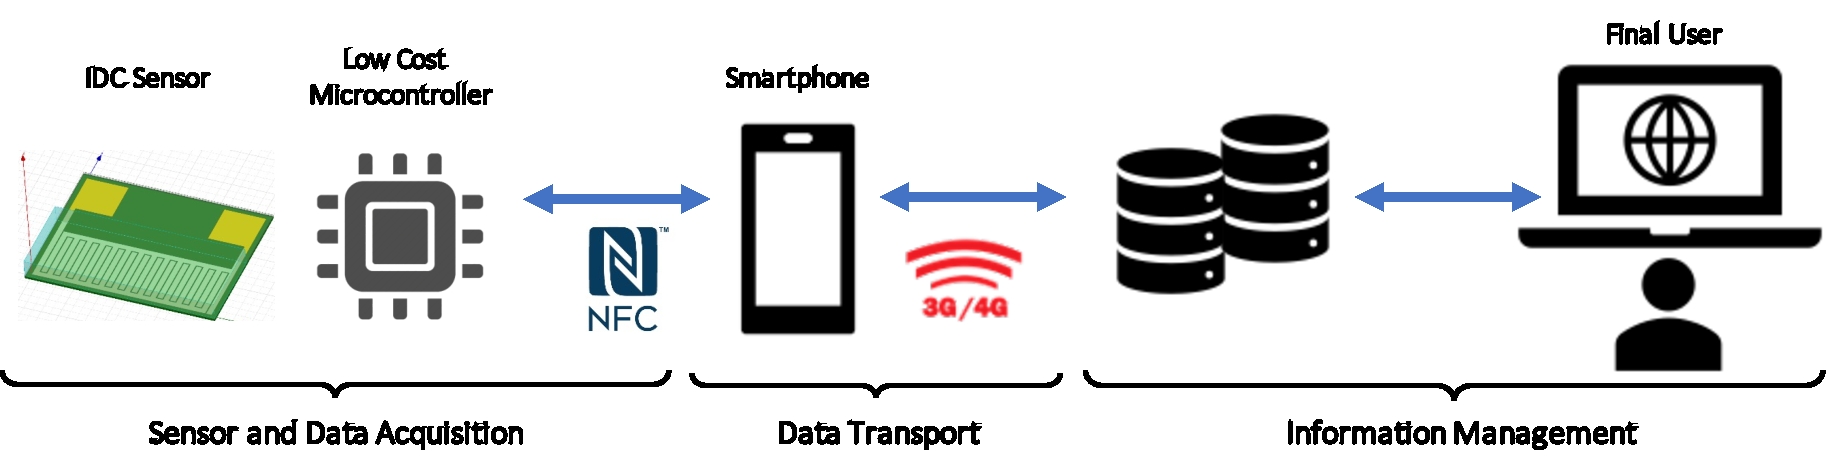
\includegraphics[width=15cm]{Cap3/arch.pdf}
\caption{Arquitectura de la solución basada en IoT.} \label{fig:arch}
\end{figure}

Se deberá privilegiar el uso de formatos vectoriales, por ejemplo pdf.


\section{Uso  de Tablas}

Cuando se requiera incluir tablas, cada columna deberá llevar un título y su correspondiente leyenda \textbf{encima de la tabla}. Como ejemplo se incluye la Tabla~\ref{tabla:capacitancia}.

\begin{table}[ht]
\begin{center}
\caption{Valor de la capacitancia utilizando sensores grandes y variando la capa aislante.}
\scalebox{1}[1]{
\begin{tabular}{| l | c | c | c|}
\hline
 \textbf{Parámetro} & \textbf{Sensor 1} & \textbf{Sensor 2} & \textbf{Sensor 3} \\
\hline
\hline
 Largo [cm] & 10.5 & 10.5 & 14 \\
%\hline
Ancho [cm] & 8 & 8 & 10.5 \\
%\hline
Aislante & Laca & Pintura & Laca \\
%\hline
Aire [nF] & $71.5\ensuremath{\times 10^{-3}}$ & 65.6 & 96.2 \\
%\hline
Agua destilada [nF] & $251\ensuremath{\times 10^{-3}}$ & 1.24 & 2.75 \\
%\hline
Concentración Tipo 1 [nF] & $358\ensuremath{\times 10^{-3}}$ & 1.8 & 140 \\
%\hline
Concentración Tipo 2 [nF] & $360\ensuremath{\times 10^{-3}}$ & 3 & 195 \\
%\hline
Concentración Tipo 3 [nF] & $380\ensuremath{\times 10^{-3}}$ &	3.2 & 228 \\
\hline
\end{tabular}}
\label{tabla:capacitancia}
\end{center}
\end{table}


\section{Uso de Ecuaciones}

Cuando se requiera, se podrán incluir ecuaciones siguiendo el ejemplo de la Ecuación~\ref{Eq1}:

\begin{equation} \label{Eq1}
k_1=\left(1+\frac{2a}{2d+b}\right) \sqrt{\frac{1+b/d}{(1+a/d+b/d)(1+a/d)}}
\end{equation}


\section{Uso de Referencias}

Cuando se deba incluir una referencia bibliográfica, se deberá incluir en el archivo \texttt{biblio.bib}, utilizando Bibtex y siguiendo el formato IEEEtrans~\cite{referencia1}.
 % max 4p
\chapter{Desarrollos}\label{tecnicas}


\begin{tcolorbox}[width=\textwidth,colback={white},title={\textbf{Lineamientos del Capítulo Desarrollos}},colbacktitle=black,coltitle=white]    
En este capítulo se deberá presentar en detalle la solución alcanzada, incluyendo todas las técnicas, mecanismos, algoritmos diseñados para resolver la problemática planteada. También se deberá presentar la metodología de diseño utilizada para alcanzar esta solución.
\end{tcolorbox}    
 % max 20p
\chapter{Experimentos y Análisis de Resultados}\label{experimentos}

\begin{tcolorbox}[width=\textwidth,colback={white},title={\textbf{Lineamientos del Capítulo Experimentos y Análisis de Resultados}},colbacktitle=black,coltitle=white]    
En este capítulo se debe presentar la configuración experimental, las pruebas propuestas y aplicadas, así como el análisis detallado de los resultados alcanzados.

\end{tcolorbox}    




 % max 10p
\chapter{Conclusiones y Trabajo Futuro}\label{concl}



\begin{tcolorbox}[width=\textwidth,colback={white},title={\textbf{Lineamientos del Capítulo Conclusiones y Trabajo Futuro}},colbacktitle=black,coltitle=white]    
Las conclusiones deben ser la respuesta a los objetivos propuestos, presentando el nivel de cumplimiento alcanzado en cada caso. 

También se puede presentar un conjunto de recomendaciones o siguientes pasos para continuar con el trabajo iniciado en el proyecto.

\end{tcolorbox}    % max 2p

%%%%%%%%%%%%%%%%%%%%%%%%%%%%%%%%%%%%%%%%%%%%%
% BIBLIOGRAFIA
%%%%%%%%%%%%%%%%%%%%%%%%%%%%%%%%%%%%%%%%%%%%%
\addcontentsline{toc}{chapter}{\numberline{}Bibliografía}
\bibliographystyle{ieeetran}
\bibliography{biblio}

%%%%%%%%%%%%%%%%%%%%%%%%%%%%%%%%%%%%%%%%%%%%%
% ANEXOS
%%%%%%%%%%%%%%%%%%%%%%%%%%%%%%%%%%%%%%%%%%%%%
\begin{appendix}
\chapter{Anexo: Nombre del Primer Anexo}\label{AnexoA}

\begin{tcolorbox}[width=\textwidth,colback={white},title={\textbf{Lineamientos del Capítulo Anexos}},colbacktitle=black,coltitle=white]    
Los anexos son opcionales, no se consideran parte central del documento y no se contarán dentro de la extensión máxima. Al ser opcionales, los anexos no pueden ser un componente fundamental en la comprensión del trabajo de grado.

\end{tcolorbox}   



\lipsum[9-10]

\chapter{Anexo: Nombre del Segundo Anexo}\label{AnexoB}

\lipsum[6-7]


\end{appendix}

\end{document}